%!TEX TS-program = xelatex
\documentclass[]{friggeri-cv}
\usepackage{afterpage}
\usepackage{hyperref}
\usepackage{color}
\usepackage{xcolor}
\usepackage{smartdiagram}
\usepackage{fontspec}
% if you want to add fontawesome package
% you need to compile the tex file with LuaLaTeX
% References:
%   http://texdoc.net/texmf-dist/doc/latex/fontawesome/fontawesome.pdf
%   https://www.ctan.org/tex-archive/fonts/fontawesome?lang=en
%\usepackage{fontawesome}
\usepackage{metalogo}
\usepackage{dtklogos}
\usepackage[utf8]{inputenc}
\usepackage{tikz}
\usetikzlibrary{mindmap,shadows}

\newcommand{\expand}[2]{\hspace*{#1}#2\hspace*{#1}}

\hypersetup{
    pdftitle={},
    pdfauthor={},
    pdfsubject={},
    pdfkeywords={},
    colorlinks=false,           % no lik border color
    allbordercolors=white       % white border color for all
}
\smartdiagramset{
    bubble center node font = \color{white}\bfseries,
    bubble node font = \color{white}\footnotesize\bfseries,
    % specifies the minimum size of the bubble center node
    bubble center node size = 0.5cm,
    %  specifies the minimum size of the bubbles
    bubble node size = 0.5cm,
    % specifies which is the distance among the bubble center node and the other bubbles
    distance center/other bubbles = 0.3cm,
    % sets the distance from the text to the border of the bubble center node
    distance text center bubble = 0.3cm,
    % set center bubble color
    bubble center node color = pblue,
    % define the list of colors usable in the diagram
    set color list = {lightgray, materialcyan, orange, materialorange, materialteal, materialindigo, materialgreen, materiallime},
    % sets the opacity at which the bubbles are shown
    bubble fill opacity = 0.7,
    % sets the opacity at which the bubble text is shown
    bubble text opacity = 0.9,
}
\tikzset{
bubble center node/.append style={text=white},
bubble node/.append style={text=white}
}

\addbibresource{bibliography.bib}
\RequirePackage{xcolor}
\definecolor{pblue}{HTML}{0395DE}

\begin{document}
\header{    CAMARENA }{Francesca}
{Robotics | Software Engineer | Mechatronics Engineer}

% % Fake text to add separator
% \fcolorbox{white}{gray}{\parbox{\dimexpr\textwidth-2\fboxsep-2\fboxrule}{%
% .....
% }}

% In the aside, each new line forces a line break
\begin{aside}
  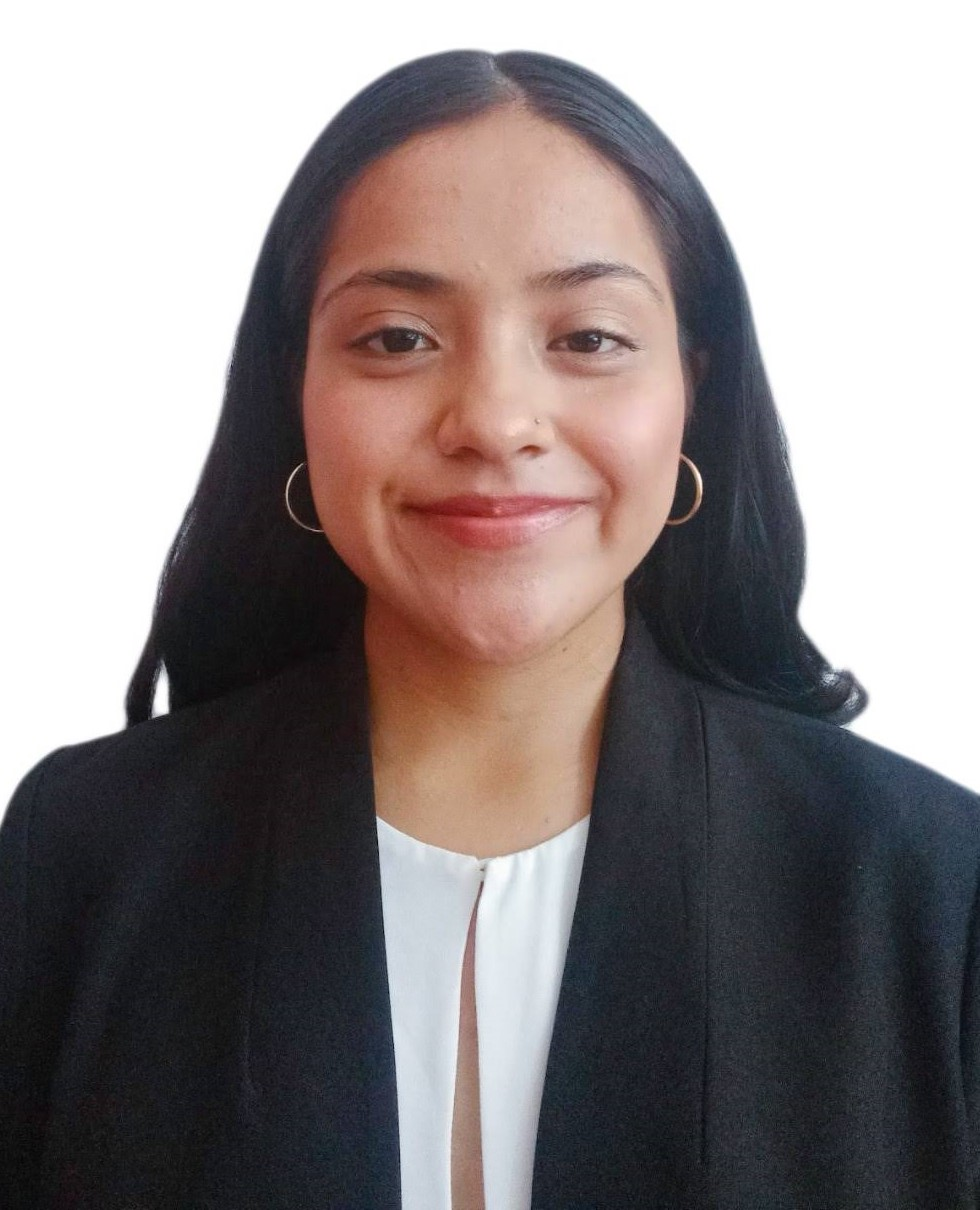
\includegraphics[scale=0.12]{img/igor}
  \section{Address}
    ~
    Paris, France
    ~
  \section{On the Web}
    ~
    \small\href{https://github.com/cuycorp}{\texttt{GitHub::cuycorp}}
    \small\href{https://www.linkedin.com/in/francesca-camarena-a26100199/}{\texttt{LinkedIn::Francesca Camarena}}
    ~
  \section{Phone}
    ~
    +33 0767124863
    ~
  \section{Mail}
    ~
    \href{mailto:14.francesca.camanrena@gmail.com}{\small\texttt{14.francesca.camanrena@gmail.com}}
    ~
  % use \expand{margin}{what}to change bubble size, if needed
  \section{Programming}
    \smartdiagram[bubble diagram]{
        \textbf{C++},
        {\expand{1mm}{Python}},
        {\expand{3mm}{C++}},
        {\expand{3mm}{C}},
        {\expand{1mm}{Typescript}},
        {\expand{1mm}{Docker}},
        {\expand{0mm}{ROS}},
        {\expand{2mm}{Linux}}}
    ~
  \section{Fields of Interest}
    \smartdiagram[bubble diagram]{
        Robotics,
        Computer Vision,
        Machine Learning,
        Localization,
        Control,
        Sim2Real
    }
    ~
  \section{Languages}
    \textbf{English [bilingual]}\includegraphics[scale=0.40]{img/5stars.png}
    \textbf{French [proficient]}\includegraphics[scale=0.40]{img/4stars.png}
    \textbf{Spanish [native]}\includegraphics[scale=0.40]{img/5stars.png}
    ~
\end{aside}
~
\section{Experience}
\begin{entrylist}
  \entry
    {02/19 - Now}
    {Senior Software Engineer for Autonomous Driving\\}
    {BMW Group, Munich, Germany}
    {I work on Obstacle Avoidance feature as part of a team. In addition to that, I am Deputy Facilitator of Software Quality community, one of a handfull of people defining standards for C++ within the company, and I wrote the library for error handling mechanism used throughout the BMW Group codebase.\\}
  \entry
    {07/17 - 12/17}
    {Robotics Software Engineer Intern}
    {\href{https://nuro.ai/}{Nuro}, Mountain View, USA}
    {I worked as part of a small perception team developing the first ever autonomous delivery bot. My work focused on LiDAR scene segmentation, sensor fusion, and sensor calibration. I was fully responsible for all software for cameras and LiDAR calibration.\\}
  \entry
    {05/14 - 02/19}
    {Research Fellow}
    {University of Bonn, Bonn, Germany}
    {I was the first student at the lab and have set up all the lab infrastructure including a full CI setup. Scientifically I have worked on various topics such as mobile robot navigation, range-based scene interpretation, and mapping. I published at top-tier international conferences such as ICRA and IROS and my code is available as open source.\\}
  \entry
    {01/12 - 05/14}
    {Research Assistant}
    {AIS lab, University of Freiburg, Freiburg, Germany}
    {As a research assistant in the Autonomous Intelligent Systems lab at the University of Freiburg, led by Prof.~Dr.~Wolfram Burdard, I dealt with Kinect RGBD sensors mounted onto various platforms. I have implemented traversability analysis for a mobile robot as part of the ROVINA project. The developments in this project led to a publication at ECMR already during my masters.\\}
  \entry
    {12/11 - 03/12}
    {Tutor, Image Processing}
    {University of Freiburg, Freiburg, Germany}
    {During my first semester I was tutoring the Image Processing course.\\}
  \entry
    {03/10 - 10/11}
    {Junior Software Engineer}
    {Timecode LLC, Kyiv, Ukraine}
    {Developed casual games for Android and a Web store for ASUS Xtion.}
\end{entrylist}
\section{Selected Projects}
\begin{entrylist}
  \entry
    {2026 - Present }
    {\href{https://github.com/cuycorp/Modern-Robot-Learning}{ | Modern Robot Learning}}
    {AI Lab - 42 AI}
    {A modular robotics research platform for learning and experimentally evaluating modern approaches to robot perception, manipulation, imitation learning, reinforcement learning, and embodied foundation models.\\\url{https://github.com/cuycorp/Modern-Robot-Learning}\\}
  \entry
    {2026 - Present }
    {\href{https://github.com/cuycorp/Duck}{ | Duck - a thought tracker}}
    {Personal project}
    {A local-first focus companion, desltop overlay application, that lets users quickly externalize distracting thoughts and return to their task.\\\url{https://github.com/cuycorp/Duck}\\}
  \entry
    {2026 - Present }
    {\href{https://github.com/lynyam/tokenscope}{ | Tokenscope}}
    {Ecole 42}
    {TokenScope is a collaborative platform that helps engineering teams understand where their LLM spending comes from by collecting usage traces, calculating estimated cost, visualizing live analytics, and generating grounded optimization recommendations.\\\url{https://github.com/lynyam/tokenscope}\\}
  \entry
    {2025 }
    {\href{https://github.com/cuycorp/minishell}{ | Minishell}}
    {Ecole 42}
    {Developing an autonomous robot for underground exploration I was responsible for traversability analysis, navigation, exploration and some of the mapping tasks. The project received excellent reviews from the EU commission.\\\url{https://github.com/cuycorp/minishell}\\}
\end{entrylist}
\newpage

\afterpage{%
\newgeometry{left=1.5cm,top=2cm,right=1.5cm,bottom=2.5cm,nohead,nofoot}
% material for this page

\section{Video Lectures on C++ on YouTube}
I have designed and released a course on Modern C++ for Image Processing. It has more than 45000 views to date and gains popularity in the robotics circles. It is available on \href{https://www.youtube.com/playlist?list=PLgnQpQtFTOGR50iIOtO36nK6aNPtVq98C}{\textbf{YouTube}} and on the website of the IPB lab:\\\url{http://www.ipb.uni-bonn.de/teaching/modern-cpp/}.

\section{First-author Publications}
 \shortentrywide
    {A general framework for flexible multi-cue photometric point cloud registration}
    {ICRA 2018}
 \shortentrywide
    {Analyzing the quality of matched 3d point clouds of objects}
    {IROS 2017}
 \shortentrywide
    {Efficient Online Segmentation for Sparse 3D Laser Scans}
    {PFG 2017}
 \shortentrywide
    {Fast range image-based segmentation of sparse 3d laser scans for online operation}
    {IROS 2016}
 \shortentrywide
    {Robust homing for autonomous robots}
    {ICRA 2016}
\shortentrywide
    {Where to Park? Minimizing the Expected Time to Find a Parking Space}
    {ICRA 2015}
\shortentrywide
    {Efficient Traversability Analysis for Mobile Robots using the Kinect Sensor}
    {ECMR 2013}

\section{Honors \& Awards}
\begin{entrylist}
  \entrywide
    {2013}
    {MINT Excellence Network Member}
    {MLP Stiftung}
    {I was chosen as one of 300 best applicants across Germany to the MINT Excellence Network.\\The candidates were chosen from the students who work in the fields of Maths, Computer Science, Natural Sciences and Tech across Germany.\\}
    {17.5cm}
  \entrywide
    {2018}
    {Best PhD Thesis of the Faculty Award}
    {University of Bonn}
    {My PhD thesis "Robot mapping and navigation in real-world environments" has been awarded the title of the best out of all written at my faculty in 2018.}
    {17.5cm}
\end{entrylist}

\section{Education}
\begin{entrylist}
  \entrywide
    {2011 - 2014}
    {MSc. Computer Software Engineering}
    {Ecole 42, France}
    {A project-based and peer-to-peer computer science program ranked the world’s 3rd most innovative university in the 2025 and 2026 WURI rankings. Training focused on system-level programming, C, Linux, Git, and shell development, with extensive team projects in an autonomous, collaborative learning environment.\\}
    {16.5cm}
  \entrywide
    {2017- 2022}
    {BSc. Mechatronics Engineering}
    {Pontifical Catholic University of Peru, Lima, Peru}
    {The Pontifical Catholic University of Peru (PUCP) is ranked No. 1 in Peru and No. 10 in Latin America. My studies focused on mechanical and electronic systems and the design of integrated hardware–software automation systems. Thesis: design of an EEG-controlled omnidirectional wheelchair..\\}
    {16.5cm}
  \entrywide
    {2015 - 2016}
    {Bilingual International Baccalaureate Diploma}
    {Newton College, Lima, Peru}
    {Top builingual Peruvian-British school, focused on developing inquisitive, outspoken and well-rounded individuals that have intercultural understanding.\\}
    {16.5cm}
\end{entrylist}

\begin{flushleft}
\emph{\today}
\end{flushleft}
\vspace{-8mm}
\begin{flushright}
\emph{CAMARENA PUCUHUANCA, Monica Francesca}
\end{flushright}

\clearpage
\restoregeometry
}


\end{document}
